\documentclass[pdf, intlimits, 9pt, unicode]{beamer}

\input{../config.tex}
\input{../header.tex}
\renewcommand{\docname}{Введение в машинное обучение}


\title[\disciplineshortname]{\docname}



\begin{document}
\frame{\titlepage}

\begin{frame}<handout:0>{Содержание}\tableofcontents[pausesections]\end{frame}

\section{Сколько всего моделей обучения?}





\begin{frame}{Зачем моделировать обучение}
Обучаемость (в приборных комплексах) можно понимать как способность применяемых алгоритмов обеспечивать {\color{red}эмпирическое обобщение}.\pause

Неформально, машинное обучение можно представить как процесс нахождения неизвестного решающего правила (или неизвестной целевой функции) по некоторой начальной информации, которая не является полной.
\end{frame}




\begin{frame}
Два основных типа проблем в математике:

\begin{enumerate}
\item {\color{red}математический анализ} -- определить математические свойства (мощность, полноту, существование решений и др.) заданных математических объектов (например, множеств, семейств функций, уравнений)\pause
\item {\color{red}математический синтез} -- найти математический объект, удовлетворяющий данным свойствам (в частности, нахождение неизвестного решающего/классифицирующего правила в задаче машинного обучения)
\end{enumerate}

% Почему на мат.анализе мы занимались сходимостью? % О... это критерий успешности для стольких процессов -- например, сходимости систем управления или сходимости экмпериментальных данных (ряда) и реализации некоторой модели

\end{frame}






\begin{frame}
\emph{Согласованной} с обучающей информацией или \emph{корректной на ней} называется любая функция, которая в точках, входящих в эту обучающую информацию, принимает точно такие же значения, какие содержатся в примерах из этой обучающей информации.

\begin{center}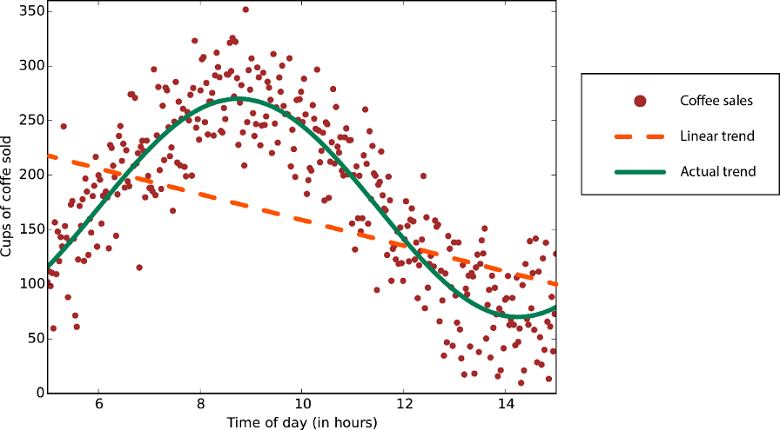
\includegraphics[height=.3\textheight]{CoffeeExample.png}\end{center}

\end{frame}




\begin{frame}<handout:0>{Пример про кофе}
\begin{center}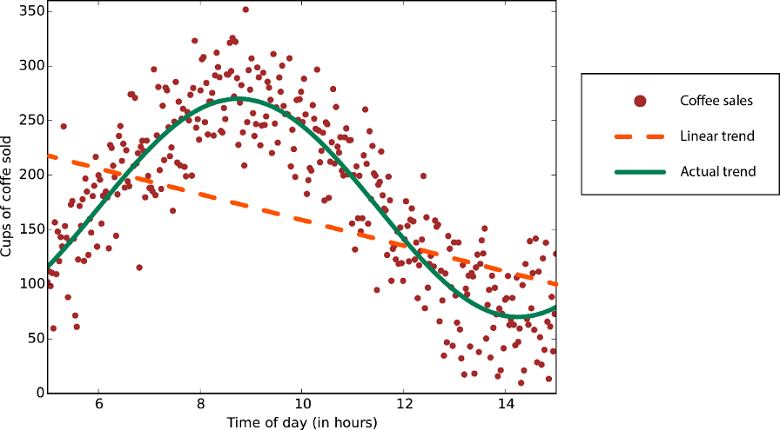
\includegraphics[width=\textwidth]{CoffeeExample.png}\end{center}
\end{frame}




\begin{frame}
В чем отличие обучения от нахождения произвольной корректной на данной обучающей информации функции?\pause

\begin{itemize}
\item Число корректных на обучающей выборке рекурсивных функций сколь угодно велико.\pause
\item Для любой обучающей выборки ограниченной длины, существует сколь угодно много корректных на этой выборке алгоритмов обучения.\pause
\item Если обучение ставит целью {\color{red}приблизить порождающую модель явления}, то истинная модель должна быть единой\pause, и решению сопутствует извлечение дополнительных сведений из/о выборке.
\end{itemize}
\end{frame}




\begin{frame}{Уточнить процесс обучения}

\begin{itemize}
\item информацию о множестве (допустимых) объектов\pause
\item о каком неизвестном решающем правиле или функции идёт речь\pause
\item что предоставляется в качестве начальной информации\pause
\item в каком классе решающих правил будет отыскиваться решение\pause
\item какие дополнительные свойства множества допустимых объектов и функций должны быть учтены\pause
%\item как будет осуществляться обучение (процесс обучения как алгоритмическое отображение начальной информации в некоторое множество решающих правил)
\item как оценивать качество обучения\pause
\item как определять, существует ли возможность достижения требуемого качества обучения при перечисленных условиях (имеет ли место обучаемость)\pause
\item как оценивать число обучающих примеров, требуемых для достижения нужного качества обучения
\end{itemize}
\end{frame}





\begin{frame}{Возможно ли обучение?}

{\color{red}Теория равномерной сходимости} (Вапника-Червоненкиса, VC dimension, VCD) -- понятие \emph{ёмкости класса решающих правил}, в котором отыскивается классифицирующий алгоритм (характеристика сложности функциональных семейств).\pause 

%Решающую функцию $h$ следует выбирать из такого класса $H$ , который удовлетворяет определённому соотношению между величиной, характеризующей {\color{red}качество приближения функции} к заданной совокупности эмпирических данных, и величиной, характеризующей {\color{red}<<сложность>> любой выбранной приближающей функции}.

{\color{red}Теория вероятно почти корректного обучения} (probably approximately correct learning, PAC) -- оценивается ёмкость класса решающих правил, берётся эмпирическая частота ошибок, формируется функционал и оценивается возможность найти обучаемую модель заданной точности в заданном классе.\pause 

%проблематика вычислительного обучения тесно связана также и с вопросам вычислительной сложности алгоритмов. \pause В теории 

{\color{red}Критерий Акаике} (Akaike's information criterion, AIC) -- критерий выбора из класса параметризованных регрессионных моделей с функцией штрафа за количество параметров.

\end{frame}





\begin{frame}{Критерии выбора/свойства модели обучения}
\begin{itemize}
\item критерий средней ошибки на контрольных данныx\pause 
\item критерий скользящего контроля (чтобы результат не зависел от дискретизации)\pause 
\item критерии непротиворечивости/помехоустойчивость (приведение к одинаковой модели по различным подвыборкам)\pause 
\item критерии регуляризации (штрафы за выход параметров алгоритма за выделенную область)\pause 
\item оценка обобщающей способности (VC, AIC, PAC, BIC)
\end{itemize}
\end{frame}








\section{Алгоритмы обучения}





\begin{frame}{Регрессионные алгоритмы}

\begin{center}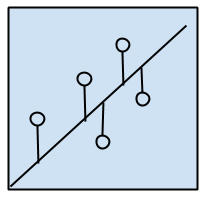
\includegraphics[height=.3\textheight]{s5-Regression-Algorithms.png}\end{center}

Регрессионный анализ -- метод моделирования измеряемых данных и исследования их свойств. \pause Данные состоят из пар значений зависимой переменной (переменной отклика) и независимой переменной (объясняющей переменной). \pause Регрессионная модель есть функция независимой переменной и параметров с добавленной случайной переменной.\pause

Регрессионным анализом называется поиск такой функции $f$, которая описывает зависимость $E(y|x) = f(x)$,  где, например, $y = f(x) + v$ ($v$ -- случайный сигнал).

\end{frame}




\begin{frame}{Регрессионные алгоритмы}
\begin{itemize}
\item Ordinary Least Squares Regression (OLSR)
\item Linear Regression
\item Logistic Regression
\item Stepwise Regression
\item Multivariate Adaptive Regression Splines (MARS)
\item Locally Estimated Scatterplot Smoothing (LOESS)
\end{itemize}
\end{frame}



\begin{frame}{Линейная регрессия}

\small

Линейная регрессия (англ. Linear regression) -- используемая в статистике регрессионная модель зависимости одной (объясняемой, зависимой) переменной y от другой или нескольких других переменных (факторов, регрессоров, независимых переменных) $x$ с линейной функцией зависимости.\pause

%Регрессионная модель

\begin{enumerate}
\item Гомоскедастичность (постоянная или одинаковая дисперсия) или отсутствие гетероскедастичности случайных ошибок модели\pause
\item Отсутствие автокорреляции случайных ошибок\pause
\item Факторы предполагаются детерминированными (нестохастическими)\pause
\item Предполагается что отсутствует полная коллинеарность факторов
\end{enumerate}


\end{frame}




%-------------------------------------

\begin{frame}{Методы на основе репрезентативных случаев (Instance-based Algorithms)}

\begin{center}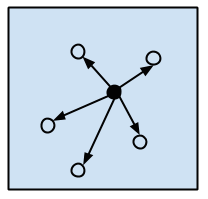
\includegraphics[height=.3\textheight]{s5-Instance-based-Algorithms.png}\end{center}

\begin{itemize}
\item k-Nearest Neighbour (kNN)
\item Learning Vector Quantization (LVQ)
\item Self-Organizing Map (SOM)
\item Locally Weighted Learning (LWL)
\end{itemize}

\end{frame}




\begin{frame}{Nearest Neighbor (Ближайший сосед)}

Метод ближайших соседей -- простейший метрический классификатор, основанный на оценивании сходства объектов. \pause Классифицируемый объект относится к тому классу, которому принадлежат ближайшие к нему объекты обучающей выборки. 

\end{frame}







%-------------------------------------

\begin{frame}{Алгоритмы регуляризации}

\begin{center}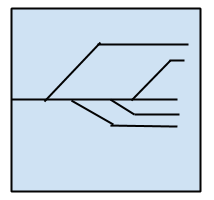
\includegraphics[height=.3\textheight]{s5-Regularization-Algorithms.png}\end{center}

\begin{itemize}
\item Ridge Regression
\item Least Absolute Shrinkage and Selection Operator (LASSO)
\item Elastic Net
\item Least-Angle Regression (LARS)
\end{itemize}

\end{frame}




%-------------------------------------

\begin{frame}{Алгоритмы с деревом принятия решений}

\begin{center}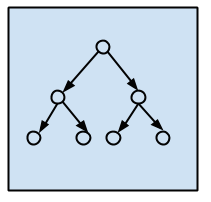
\includegraphics[height=.3\textheight]{s5-Decision-Tree-Algorithms.png}\end{center}

\begin{itemize}
\item Classification and Regression Tree (CART)
\item Iterative Dichotomiser 3 (ID3)
\item C4.5 and C5.0 (different versions of a powerful approach)
\item Chi-squared Automatic Interaction Detection (CHAID)
\item Decision Stump
\item M5
\item Conditional Decision Trees
\end{itemize}

\end{frame}




\begin{frame}{Дерево принятия решений\\(дерево классификации, регрессионное дерево)}

\small
Средство поддержки принятия решений, использующееся в статистике и анализе данных для прогнозных моделей.\pause

Структура дерева представляет собой {\color{red}<<листья>> и <<ветки>>}. \pause На ребрах (<<ветках>>) дерева решения записаны атрибуты, от которых зависит целевая функция, в <<листьях>> записаны значения целевой функции, а в остальных узлах -- атрибуты, по которым различаются случаи.\pause 

Чтобы классифицировать {\color{red}новый случай}, надо спуститься по дереву до листа и выдать соответствующее значение.\pause 

Широко используются в интеллектуальном анализе данных. \pause Цель состоит в том, чтобы создать модель, которая предсказывает значение целевой переменной на основе нескольких переменных на входе.

\end{frame}



%-------------------------------------

\begin{frame}{Байесовские алгоритмы}

\begin{center}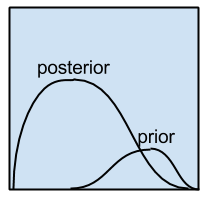
\includegraphics[height=.3\textheight]{s5-Bayesian-Algorithms.png}\end{center}

\begin{itemize}
\item Naive Bayes
\item Gaussian Naive Bayes
\item Multinomial Naive Bayes
\item Averaged One-Dependence Estimators (AODE)
\item Bayesian Belief Network (BBN)
\item Bayesian Network (BN)
\end{itemize}

\end{frame}

\begin{frame}{Bayesian Network}

Байесовский классификатор -- простой вероятностный классификатор, основанный на применении Теоремы Байеса со строгими (наивными) предположениями о независимости.\pause

\begin{itemize}
\item Могут обучаться очень эффективно \pause %\pause Во многих практических приложениях, для оценки параметров для наивных байесовых моделей используют метод максимального правдоподобия; можно работать с наивной байесовской моделью, \emph{<<не веря>>} в байесовскую вероятность и не используя байесовские методы.\pause
\item Несмотря на наивный вид и очень упрощённые условия, БК часто отлично работают во многих сложных ситуациях.\pause
\item малое количество данных для обучения, необходимых для оценки параметров, требуемых для классификации.
\end{itemize}

\end{frame}





%-------------------------------------

\begin{frame}{Алгоритмы кластеризации}

\begin{center}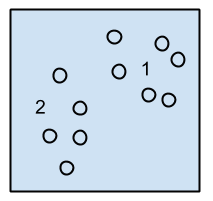
\includegraphics[height=.3\textheight]{s5-Clustering-Algorithms.png}\end{center}

\begin{itemize}
\item k-Means
\item k-Medians
\item Expectation Maximisation (EM)
\item Hierarchical Clustering
\end{itemize}

\end{frame}






\begin{frame}{Метод опорных векторов (SVM, support vector machine)}

\small

Набор алгоритмов обучения с учителем, использующихся для задач классификации и регрессионного анализа. \pause Принадлежит к семейству линейных классификаторов, может также рассматриваться как специальный случай регуляризации по Тихонову. \pause %Непрерывное уменьшение эмпирической ошибки классификации и увеличение зазора, поэтому метод также известен как метод классификатора с максимальным зазором.\pause

Основная идея -- {\color{red}перевод исходных векторов в пространство более высокой размерности} и поиск разделяющей {\color{red}гиперплоскости} с максимальным зазором в этом пространстве. \pause %Две параллельных гиперплоскости строятся по обеим сторонам гиперплоскости, разделяющей классы. \pause Разделяющей гиперплоскостью будет гиперплоскость, максимизирующая расстояние до двух параллельных гиперплоскостей. \pause Алгоритм работает в предположении, что чем больше разница или расстояние между этими параллельными гиперплоскостями, тем меньше будет средняя ошибка классификатора.
\end{frame}








%-------------------------------------

\begin{frame}{Обучение по ассоциативным правилам}

\begin{center}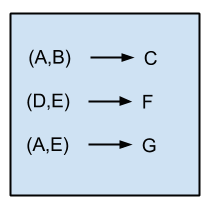
\includegraphics[height=.3\textheight]{s5-Assoication-Rule-Learning-Algorithms.png}\end{center}

\begin{itemize}
\item Apriori algorithm
\item Eclat algorithm
\end{itemize}

\end{frame}




%-------------------------------------

\begin{frame}{Искусственные нейронные сети}

\begin{center}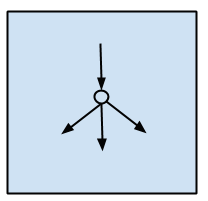
\includegraphics[height=.3\textheight]{s5-Artificial-Neural-Network-Algorithms.png}\end{center}

\begin{itemize}
\item Perceptron
\item Back-Propagation
\item Hopfield Network
\item Radial Basis Function Network (RBFN)
\end{itemize}

\end{frame}





\begin{frame}{Искусственная нейронная сеть}

\small

Искусственные нейронная сеть (artificial neural network, ANN, нейронная сеть) -- это математическая модель, а также её программные или аппаратные реализации, построенная в некотором смысле по образу и подобию сетей нервных клеток живого организма.\pause

{\color{red}ИНС} представляют собой систему соединённых и взаимодействующих между собой простых процессоров (искусственных нейронов). \pause

Такие процессоры обычно довольно просты (особенно в сравнении с процессорами, используемыми в персональных компьютерах). \pause Каждый процессор подобной сети имеет дело только с сигналами, которые он периодически получает, и сигналами, которые он периодически посылает другим процессорам. \pause И, тем не менее, будучи соединёнными в достаточно большую сеть с управляемым взаимодействием, такие локально простые процессоры вместе способны выполнять довольно сложные задачи.

\end{frame}


%-------------------------------------

\begin{frame}{Алгоритмы глубокого обучения (Deep learning)}

\begin{center}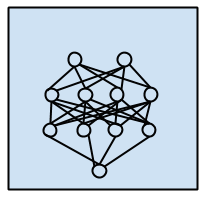
\includegraphics[height=.3\textheight]{s5-Deep-Learning-Algorithms.png}\end{center}

\begin{itemize}
\item Deep Boltzmann Machine (DBM)
\item Deep Belief Networks (DBN)
\item Convolutional Neural Network (CNN)
\item Stacked Auto-Encoders
\end{itemize}

\end{frame}




%-------------------------------------

\begin{frame}{Алгоритмы уменьшения размерности}

\begin{center}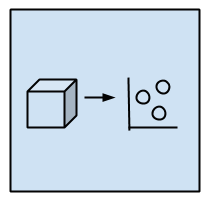
\includegraphics[height=.3\textheight]{s5-Dimensional-Reduction-Algorithms.png}\end{center}

\begin{itemize}
\item Principal Component Analysis/Regression (PCA,PCR)
\item Partial Least Squares Regression (PLSR)
\item Sammon Mapping
\item Multidimensional Scaling (MDS)
\item Projection Pursuit
\item Linear/Misture Discriminant Analysis (LDA, MDA)
\item Quadratic/Flexible Discriminant Analysis (QDA, FDA)
\end{itemize}

\end{frame}





%-------------------------------------

\begin{frame}{Ансамблевые алгоритмы (развитие деревьев)}

\begin{center}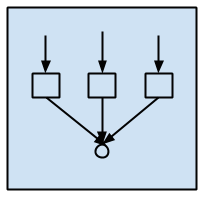
\includegraphics[height=.3\textheight]{s5-Ensemble-Algorithms.png}\end{center}

\begin{itemize}
\item Boosting
\item Bootstrapped Aggregation (Bagging)
\item AdaBoost
\item Stacked Generalization (blending)
\item Gradient Boosting Machines (GBM)
\item Gradient Boosted Regression Trees (GBRT)
\item {\color{red}Random Forest}
\end{itemize}

\end{frame}





\begin{frame}
\begin{center}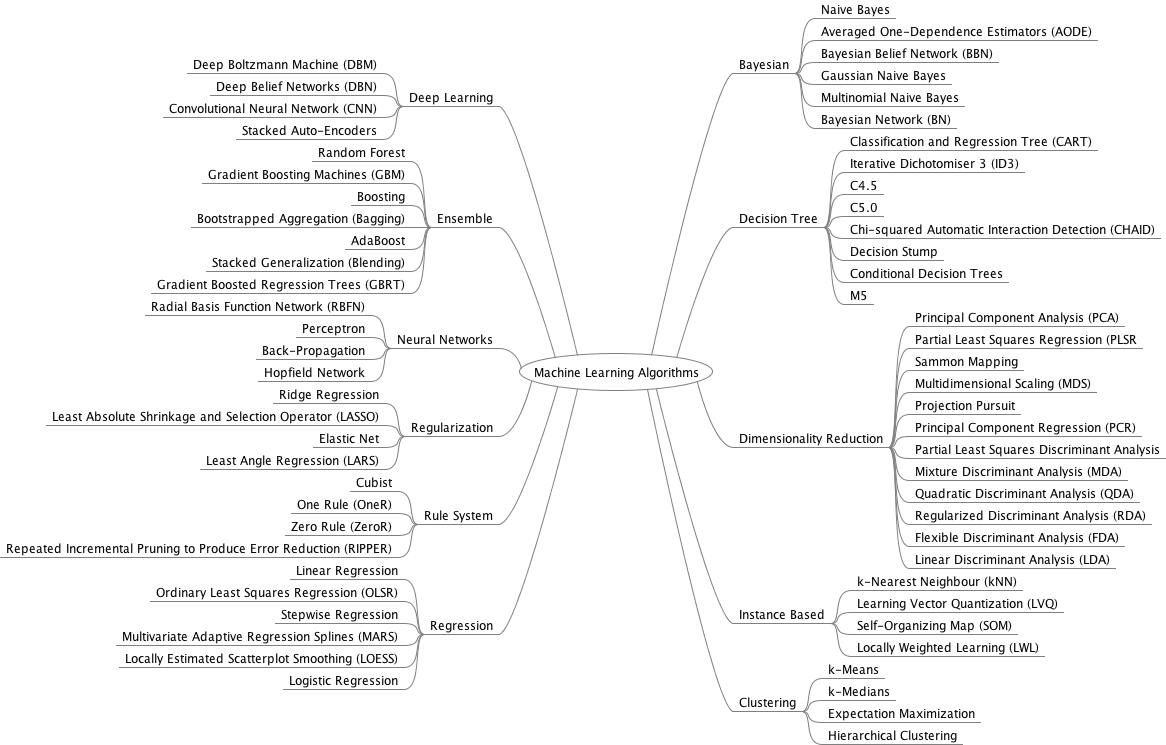
\includegraphics[width=\textwidth]{MachineLearningAlgorithms.png}\end{center}
\end{frame}









\section{Выбор модели}


\begin{frame}

1. Machine\_learning [Электронный ресурс] // Википедия : свободная энцикл. -- Электрон. дан. -- [Б. м.], 2015. -- URL: \url{http://en.wikipedia.org/wiki/Machine\_learning} (дата обращения: 11.11.2015).\\

\begin{center}\only<1>{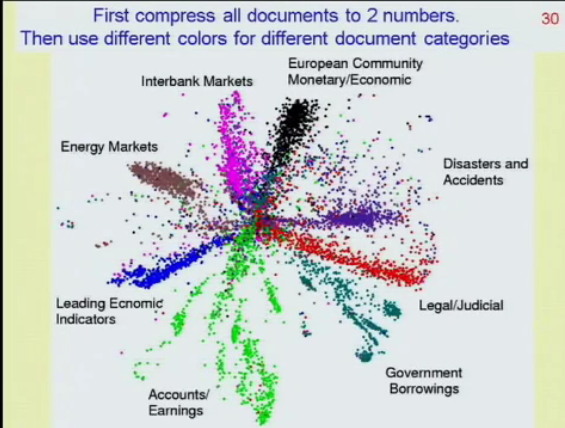
\includegraphics[height=.6\textheight]{s1.png}}\only<2>{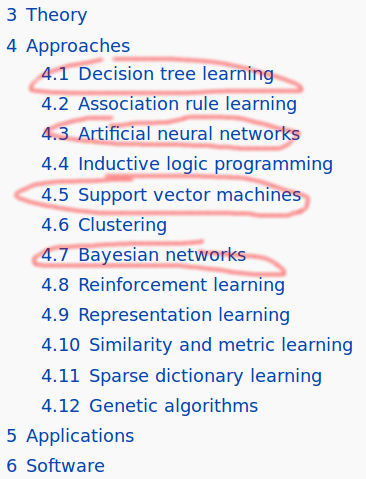
\includegraphics[height=.6\textheight]{s1_1.png}}\hspace{1cm}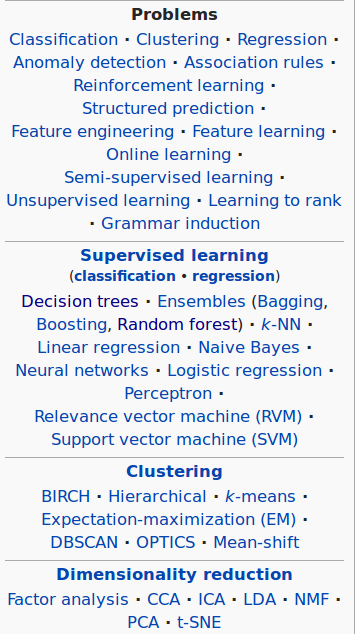
\includegraphics[height=.6\textheight]{s3.png}\end{center}
\end{frame}



% Microsoft Machine Learning Cheatsheet for MS Azure
\begin{frame}
\begin{center}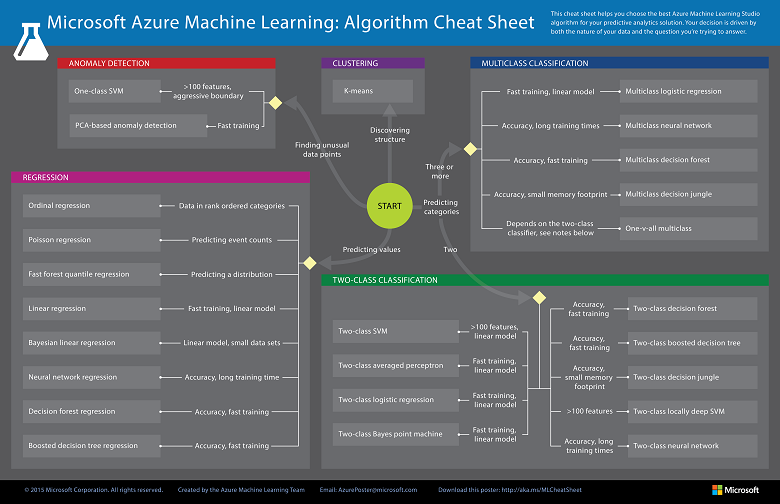
\includegraphics[height=.8\textheight]{MSMLcheatsheet.png}\end{center}
\end{frame}






























% silhouette metric
% some measure of the entropy

% traditional transductive / semi-supervised learning fails--we need to have some global information about the underlying distribution to apply these methods

% The RBM solves this problem by selecting features and forming clusters at different levels of scale, and insisting that they all be consistent.    So the RBM is internally self-consistant, thereby avoiding the need for an external cluster metric.





\stepcounter{section}
\repeatSectionTitle[Спасибо за внимание!]

\end{document}
